
\section{Integration by Parts}\label{ibp}

Integration \integ{by parts} (IBP) is the Product Rule spun around backwards to become a rule for antiderivatives rather than derivatives.  

\begin{exercise}{Reversing the Product Rule \Coffeecup \Coffeecup }
Fill in the blanks in the following construction of \antider{integration by parts}:
\begin{itemize}
\item Recall the Product Rule for derivatives. $$\left( f(x)g(x) \right)'=\hspace{3in} $$
\solushun{$$\left( f(x)g(x) \right)'=f'(x)g(x)+f(x)g'(x)$$}{0in}
\item Take an antiderivative of both sides.
$$ \hspace{2in} = \int \left( f'(x)g(x) \right) \dif x + \int \left( f(x)g'(x) \right) \dif x$$
\solushun{$$ f(x)g(x) = \int \left( f'(x)g(x) \right) \dif x + \int \left( f(x)g'(x) \right) \dif x$$}{0in}
\item Rewrite the equation by subtracting the term $\int \left( f'(x)g(x) \right) \dif x$ from both sides.

$$ = $$
\solushun{$$ f(x)g(x) - \int \left( f'(x)g(x) \right) \dif x = \int \left( f(x)g'(x) \right) \dif x$$}{0in}

\item To condense the notation, it is customary to make the substitutions $u=f(x)$ and $v=g(x)$.  Thus, we say $\frac{\dif u}{\dif x}=f'(x) $ and similarly $\frac{\dif v}{\dif x}=g'(x) $.  Multiply the $\dif x$ to the right-hand side in both of those equations, we obtain

$$\dif u = \hspace{3in} $$ and $$ \dif v = \hspace{3in}  $$

\solushun{$\dif u = f'(x)\dif x $ and $ \dif v = g'(x) \dif x$\\}{0in}

\item Use these substitutions to replace all instances of $x, f, $ and $g$ by $u$ and $v$ and conclude the IBP formula.
\solushun{$$uv-\int v\dif u=\int u\dif v$$\\}{1in}

\end{itemize}
\end{exercise}

Just for sake of having it in its own box, here it is again!
\FormulaBox{Integration by Parts Formula}{\begin{tabular}{c}
		$\int u\dif v=uv-\int v\dif u$
	\end{tabular}}
    
 We typically use this to integrate a product of functions in the case that $u$-substitution does not work.  You can identify one factor of your integrand as $u$, the remaining factor as $\dif v$, and plug into the IBP formula.  There are three main types:

\begin{enumerate}
\item A product with one factor that becomes much simpler upon differentiation
\item A not-quite-a product that we turn into a product
\item An integrand that reappears after applying IBP
\end{enumerate} We illustrate each of these methods with an example.

\subsection{A Product with One Factor That Becomes Much Simpler Upon Differentiation}\label{simpleproduct}  We let $u$ be whichever factor becomes simpler when it is differentiated.  The other factor by default must then be set equal to $\dif v$.  
%\todo[inline]{In a previous example/exercise you did not put a cdot between x and cosine. Below you do.}
%I think this is fine... here I'm specifically drawing attention to the fact that it's a product for sake of IBP
\begin{example}{Integrating a Product}\label{ucosu}
  Suppose we wish to find an antiderivative for the function $x\cdot \cos(x)$.  We can either choose $u=x$ or $u=\cos(x)$.  Since $u=x$ has lovely little constant function 1 as its derivative, whereas $u=\cos(x)$ would produce just another trig function as its derivative, we conclude $u=x$ is the better choice.  

\FormulaBox{Choice of $u$ and $\dif v$}{\begin{tabular}{c|c} 
 $u=x$ &  $v=\sin(x)$ \\ \hline
 $\dif u= \dif x$ & $\dif v=\cos(x)\dif x$ \\ 
\end{tabular}
}

We are now ready to calculate the antiderivative via IBP:
$$\int x\cdot \cos(x) \dif x = \int u \dif v = uv-\int v \dif u = x\cdot \sin(x) - \int \sin(x) \dif x = x\cdot \sin(x) +\cos(x)+C$$

\end{example}

\begin{exercise}{Checking Our Work \Coffeecup}
Take the derivative of our result,  $x \sin(x) +\cos(x)+C$, to verify that it is in fact the correct antiderivative!
\solushun{$$\frac{\dif}{\dif x}\left(x \sin(x) +\cos(x)+C\right) = x\cos(x)+\sin(x)-\sin(x)=x\cos(x)$$}{1.5in}
\end{exercise}

\begin{exercise}{An Integral via both $u$-sub and IBP \Coffeecup \Coffeecup \Coffeecup} Consider the integral $$\int x\sqrt{x+1} \dif x $$
\begin{itemize}
\item Evaluate the integral using the $u$-sub $u=x+1$.
\solushun{Letting $u=x+1$, then $\dif u = \dif x$.
\begin{align*}
\int (u-1)\sqrt{u} \dif x &= \int u^{\frac{3}{2}}-u^\frac{1}{2} \dif u \\
&=\frac{2}{5}u^{\frac{5}{2}}-\frac{2}{3}u^{\frac{3}{2}} \\
&=\frac{2}{5}(x+1)^{\frac{5}{2}}-\frac{2}{3}(x+1)^{\frac{3}{2}} \\
\end{align*}}{2in}
\item Evaluate the integral using IBP, choosing $u=x$ and $\dif v = \sqrt{x+1} \dif x$.
\solushun{Letting $u=x$ and $\dif v = \sqrt{x+1}$, then $\dif u = \dif x$ and $v = \frac{2}{3}(x+1)^\frac{3}{2}$.
\begin{align*}
\int u \dif v &= uv -\int v\dif u \\
&= x\frac{2}{3}(x+1)^\frac{3}{2} -\frac{2}{3}\int (x+1)^\frac{3}{2}\dif x \\
&= \frac{2}{3}x(x+1)^\frac{3}{2} -\frac{2}{3}\left( \frac{5}{2}(x+1)^\frac{5}{2}\right) \\
&= \frac{2}{3}x(x+1)^\frac{3}{2} -\frac{4}{15}(x+1)^\frac{5}{2} \\
\end{align*}}{2in}
\item Your answers will appear very different!  Is one incorrect?  Or are they compatible?
\solushun{
Starting with the first solution from the $u$-sub:
\begin{align*}
\frac{2}{5}(x+1)^{\frac{5}{2}}-\frac{2}{3}(x+1)^{\frac{3}{2}}&=(x+1)^\frac{3}{2}\left(\frac{2}{5}(x+1) -\frac{2}{3}\right)\\
&=(x+1)^\frac{3}{2}\left(\frac{2}{5}x+\frac{2}{5} -\frac{2}{3}\right) \\
&=(x+1)^\frac{3}{2}\left(\frac{2}{5}x -\frac{4} {15}\right) \\
\end{align*}
\\
Starting with the IBP solution:
\begin{align*}
\frac{2}{3}x(x+1)^\frac{3}{2} -\frac{4}{15}(x+1)^\frac{5}{2} &= (x+1)^\frac{3}{2}\left(\frac{2}{3}x -\frac{4}{15}(x+1) \right)\\
&= (x+1)^\frac{3}{2}\left(\frac{2}{3}x -\frac{4}{15}x-\frac{4}{15} \right)\\
&=(x+1)^\frac{3}{2}\left(\frac{2}{5}x -\frac{4} {15}\right) \\
\end{align*}}{2in}
\AnswerKeyEntry{By factoring out the quantity $(x+1)^{3/2}$, both answers can be brought into the form $(x+1)^{3/2}\left(\frac{2}{5}x-\frac{4}{15}\right)+C$.}
\end{itemize}
\end{exercise}

\subsection{A Not-Quite-a Product That We Turn into a Product} Often, an integrand that does not appear to be a product can be rewritten as product in a helpful way.  This often includes {\bf rewriting the integrand as the integrand times one}.  We let $u$ be the entire integrand, leaving $\dif v$ to just be the invisible 1 times $\dif x$.

\begin{example}{Multiplying by 1 in an IBP}
 Suppose we wish to find an antiderivative for the function $\arccos(x)$.  We identify $u=\arccos(x)$ which leaves $\dif v=1\cdot \dif x$.  Thus we make the following declarations:
\FormulaBox{Choice of $u$ and $\dif v$}{\begin{tabular}{c|c} \hline
 $u=\arccos(x)$ &  $v=x$ \\ \hline
 $\dif u=-\frac{1}{\sqrt{1-x^2}}\dif x$ & $\dif v=1\cdot \dif x$ \\ \hline
\end{tabular}}

We are now ready to calculate the antiderivative via IBP:
$$\int \arccos(x)\cdot 1 \cdot \dif x = \int u \dif v = uv-\int v \dif u = x\cdot \arccos(x) - \int x \left( -\frac{1}{\sqrt{1-x^2}} \right) \dif x $$

$$= x\arccos(x) + \int \frac{x}{\sqrt{1-x^2}} \mathtt{dx}=x\arccos(x)-\sqrt{1-x^2}+C $$

\end{example}

\begin{exercise}{Filling in the Details \Coffeecup \Coffeecup}
Notice that the very last step of the above example was in fact a $u$-substitution!  Show the details of how that antiderivative was carried out.

$$\int \frac{x}{\sqrt{1-x^2}}\dif x =\hspace{3in}$$
\solushun{Let $u=1-x^2$. Then $\dif u = -2x \dif x$.
\begin{align}
\int \frac{x}{\sqrt{1-x^2}} \dif x &=-\frac{1}{2}\int \frac{\dif u}{\sqrt{u}} \\
&= -\frac{1}{2}\int u^{-\frac{1}{2}}\dif u \\
&= -\frac{1}{2}\cdot 2 u^{\frac{1}{2}} + C \\
&= -(1-x^2)^{\frac{1}{2}} + C \\
&= -\sqrt{1-x^2} + C \\
\end{align}}{1.5in}
\AnswerKeyEntry{Use the substitution $u=1-x^2$.}
\end{exercise}

\begin{exercise}{The Antiderivative of the Natural Logarithm \Coffeecup \Coffeecup}
Apply the same technique to find an \logarithms{antiderivative} for the function $\ln(x)$.
\solushun{Let $u=\ln(x)$ and $\dif v = 1 \dif x$. Then $\dif u = \frac{1}{x} \dif x$ and $v = x$.
\begin{align}
\int \ln(x) \dif x &= x\ln(x) -\int x \frac{1}{x} \dif x \\
&= x\ln(x)-\int \dif x \\
&= x\ln(x)-x+C \\
\end{align}}{2in}
\AnswerKeyEntry{The antiderivative is $x\ln(x)-x+C$.}
\end{exercise}

\subsection{An Integrand that Reappears After Applying IBP}\label{reappear} Sometimes, we can get the original expression to come back after applying integration by parts one or more times.  Once this occurs, you can {\bf give some name to the integral (we will use $I$)} and solve for it as you would solve any equation in algebra!

\begin{example}{An Integrand that Reappears After IBP}
Suppose we wish to find an antiderivative for the function $e^{2x}\cos(x)$.  Call $I$ the desired antiderivative.  That is:

$$ I=\int e^{2x}\cos(x) \dif x$$ 

We now wish to apply IBP, so we make the following declarations:
\FormulaBox{Choice of $u$ and $\dif v$}{\begin{tabular}{c|c} 
 $u=e^{2x}$ &  $v=\sin(x)$ \\ \hline
 $\dif u=2e^{2x}\dif x$ & $\dif v=\cos(x) \dif x$ \\ 
\end{tabular}
}

We are now ready to calculate the antiderivative via IBP:
\begin{align*} I &= \int u \dif v \\
&= uv-\int v \dif u \\ 
&= e^{2x}\sin(x) - \int \sin(x) \cdot 2e^{2x} \dif x \\
&= e^{2x}\sin(x) -2 \int e^{2x}\sin(x) \dif x \\
\end{align*}

We notice now that the new integral is again a product of functions (and does not appear to be doable via $u$-sub) so we apply IBP once again with the following declarations (using new $u$ and $v$):
\FormulaBox{Choice of $u$ and $\dif v$}{\begin{tabular}{c|c} 
 $u=e^{2x}$ &  $v=-\cos(x)$ \\ \hline
 $\dif u=2e^{2x}\dif x$ & $\dif v=\sin(x) \dif x$ \\ 
\end{tabular}
}

We now proceed with the previous expression, using the new IBP setup and notice that the original integral $I$ reappears:

\begin{align*} I &= e^{2x}\sin(x) -2 \int u \dif v \\
&=e^{2x}\sin(x) -2 \left( uv-\int v \dif u \right) \tag{$\bowtie$} \\
&=e^{2x}\sin(x) -2 \left( e^{2x}(-\cos(x))-\int (-\cos(x))2e^{2x} \dif x \right) \tag{$\bowtie$} \\
&=e^{2x}\sin(x) +2e^{2x}\cos(x)-4\int e^{2x}\cos(x) \dif x \\
&=e^{2x}\sin(x) +2e^{2x}\cos(x)-4I
\end{align*}

At first glimpse this seems troubling; we have reduced the problem we are trying to solve to solving the exact same problem that we are trying to solve!  Yet upon further inspection, it becomes clear that this is in fact an equation involving $I$, and thus we can solve for it!  Proceeding: 

\begin{align*} I&=e^{2x}\sin(x) +2e^{2x}\cos(x)-4I \\
5I&=e^{2x}\sin(x) +2e^{2x}\cos(x) \\
I&=\frac{e^{2x}\sin(x) +2e^{2x}\cos(x)}{5}
\end{align*} and we are done, concluding that $$ \int e^{2x}\cos(x) \dif x=\frac{e^{2x}\sin(x) +2e^{2x}\cos(x)}{5}+C$$

\end{example}

\begin{exercise}{Carefulness \Coffeecup}
In the example above, there are two lines labeled with bowties ($\bowtie$).  Explain briefly in a sentence or two why those giant parentheses are present.  What would go wrong if those parentheses were not there?
\solushun{When IBP is used to evaluate an antiderivative, it is important to distribute the integral's coefficient to both parts of the new expression. If the parentheses weren't there, the coefficients would only be applied to the first expression in each IBP expansion.\\}{1in}
\end{exercise}


\begin{example}{Another Reappearing IBP Integral}\label{AnotherReappearing}
 Suppose we wish to find an antiderivative for the function $\tan(x)\sec^2(x)$.  We identify $\dif v=\sec^2(x) \dif x$ as having a nice clean antiderivative, which leaves $u=\tan(x)$ by default.  Thus we make the following declarations:

\FormulaBox{Choice of $u$ and $\dif v$}{\begin{tabular}{c|c} \hline
 $u=\tan(x)$ &  $v=\tan(x)$ \\ \hline
 $\dif u=\sec^2(x)\dif x$ & $\dif v=\sec^2(x) \dif x$ \\ 
\end{tabular}
}

We are now ready to calculate the antiderivative via IBP:
$$\int \tan(x)\sec^2(x) \dif x = \tan(x)\tan(x) - \int \tan(x) \sec^2(x)\dif x $$

We notice that the original integral has reappeared!  We give it the name $I$ and solve.  The equation becomes $I = \tan^2(x) - I$, which implies that $2I=\tan^2(x)$.  Dividing by two produces the following result:

$$\int \tan(x)\sec^2(x) \dif x =\frac{1}{2}\tan^2(x)+C$$

\end{example}

\begin{exercise}{Alternate Solutions \Coffeecup \Coffeecup }
Find the antiderivative of $\tan(x)\sec^2(x)$ yet again but by two different methods!  In particular, try...
\begin{itemize}
\item ...a $u$-sub with $u=\tan(x)$. \vspace*{1.5in}
\item ...an IBP with $u=\sec(x)$ and $\dif v = \tan(x)\sec(x) \dif x$. \vspace*{1.5in}
\end{itemize}
Confirm that your answers match the result of Exercise \ref{reappear}.\ref{AnotherReappearing}.
\end{exercise}

\begin{exercise}{A Tricky but Important One: Secant \secant{Cubed} \Coffeecup \Coffeecup \Coffeecup }\label{seccubed}
  Find an antiderivative for the function $\sec^3(x)$.  ({\bf Hint:} Split the cube as $\sec^3(x)=\sec^2(x)\sec(x)$.  Also, the \trigidentities{Pythagorean Identity} $\tan^2(x)=\sec^2(x)-1$ will be useful.)
\solushun{Let $I$ = $\int\sec^3(x) \dif x$ then split the integral:
$$\int \sec^3x \dif x = \int \sec x \sec^2x \dif x$$
Then, let $u=\sec x$ and $\dif v = \sec^2x$. Then $\dif u = \sec x \tan x \dif x$ and $v = \tan x$. 
\begin{align*}
I = \int \sec x \sec^2x \dif x &= \sec x \tan x-\int\tan x \cdot \sec x \tan x \dif x \\
&= \sec x \tan x-\int\tan^2 x \sec x  \dif x \\
&= \sec x \tan x-\int\left(sec^2x-1\right) \sec x  \dif x \\
&= \sec x \tan x-\int \sec^3 x-\sec x  \dif x \\
&= \sec x \tan x-\left(\int \sec^3 x\dif x-\int\sec x  \dif x\right) \\
&= \sec x \tan x-\int \sec^3 x\dif x+\ln|\sec x + \tan x|+C   \\
I &= \sec x \tan x-I+\ln|\sec x + \tan x|+C   \\
2I &= \sec x \tan x+\ln|\sec x + \tan x|+C   \\
I &= \frac{\sec x \tan x+\ln|\sec x + \tan x|}{2} + C
\end{align*}}{4in}
\AnswerKeyEntry{The antiderivative is $\frac{1}{2}\left(\sec(x)\tan(x)+\ln|\sec(x)+\tan(x)|\right)+C$.}
\end{exercise}
\begin{comment}
\subsection{Spot the Error!}
\todo[inline]{I think I'm actually going to put alllll of the STE's at the very end of the section as one big mixed region.}
\todo[inline]{I kind of like that idea. Sort of a review section of mixed practice. Don't tell them what method to use, have spot the errors... Be a good place for old midterm/final problems that you never want to use again.}
In each of the following attempted solutions, there is an error.  Circle where the error occurs and write a short sentence that describes what went wrong.  \begin{enumerate}
\item Find the antiderivative: $ \int \frac{x}{x^2+1} \dif x $
\begin{center}
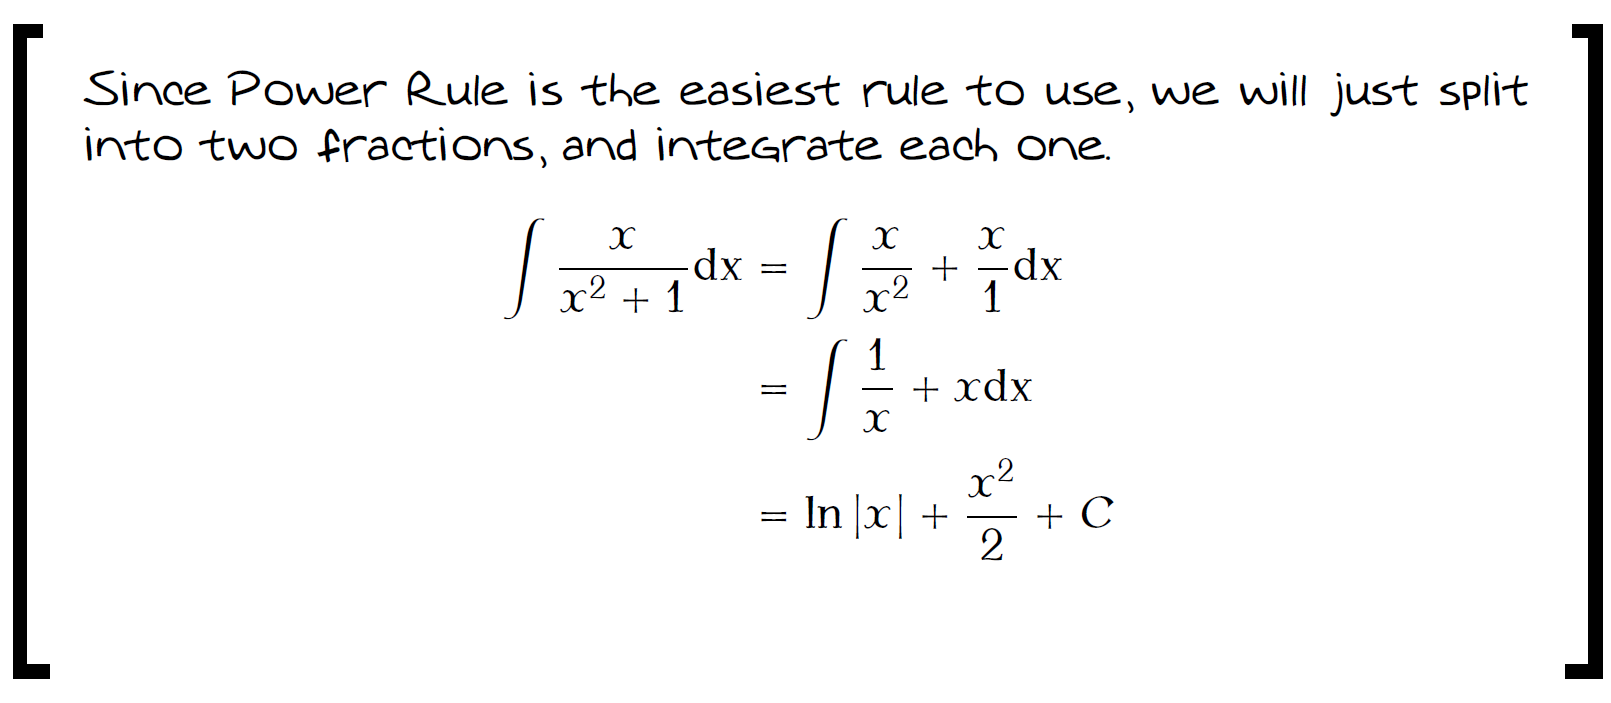
\includegraphics[scale=0.35]{ChapterAntidiff/STEusub.png}
\end{center}

\item Find the antiderivative: $\int x^2\cos(2x) \dif x$
\end{enumerate}

\end{comment}
\section{Mixed Practice with Substitution/IBP}

Sometimes it is not obvious which technique to use in solving a particular problem.  One must often use more than one technique of integration in combination. 

\begin{exercise}{Practice on $u$-sub and/or IBP \Coffeecup \Coffeecup \Coffeecup}
\begin{itemize}
\item Find an antiderivative for the function $\cos(\sqrt{x})$.
\solushun{Start with a $u$-sub. Let $u=\sqrt{x}$. Then $\dif u = \frac{1}{2\sqrt{x}}\dif x$ and $\dif x = 2\sqrt{x}\dif u$
\begin{align*}
\int\cos\sqrt{x}\dif x =\int\cos u\cdot2u\dif u &= 2\int u\cos u\dif u \\
&=2\left(u\sin u + \cos u +C \right) \text{, Example \ref{simpleproduct}.\ref{ucosu}} \\
&=2\sqrt{x}\sin \left(\sqrt{x}\right) + 2\cos\left(\sqrt{x}\right) +C 
\end{align*}}{2in}

\item Evaluate $\int e^{\sqrt{2x}} \dif x$.
\solushun{Start with a $u$-sub. Let $u=\sqrt{2x}$. Then $\dif u = \frac{1}{\sqrt{2x}}\dif x$ and $\dif x = \sqrt{2x}\dif u$
$$\int e^{\sqrt{2x}} \dif x =\int e^{u}\cdot \sqrt{2x} \dif u = \int ue^{u}\dif u $$
Then, proceed with an IBP, using $u=u$, $\dif v=e^u\dif u$, $\dif u=\dif u$, and $v=e^u$.
\begin{align*}
\int ue^{u}\dif u &= ue^u-\int e^{u} \dif u  \\
&=ue^u-e^u +C\\
&=e^u\left(u-1\right) +C\\
&=e^{\sqrt{2x}}\left(\sqrt{2x}-1\right)+C
\end{align*}}{2in}

\item Evaluate $\int \arcsin(5x) \dif x$.
\solushun{Start with a $u$-sub. Let $u=5x$, $\dif u = 5\dif x$:
$$\int\arcsin(5x)\dif x=\frac{1}{5}\int\arcsin(u)\dif u$$
Then, use IBP (we'll use $p,q$ in place of $u,v$ to avoid confusion):
Let $p=\arcsin(u)$ and $\dif q = \dif u$, then $\dif p = \frac{1}{\sqrt{1-u^2}}\dif u$ and $q=u$:

$$\frac{1}{5}\int\arcsin(u)\dif u=\frac{1}{5}\left(u\arcsin(u)-\int\frac{u}{\sqrt{1-u^2}}\dif u\right)$$

Then, we apply another $u$-sub (we will use $v$ to avoid confusion), with $v=1-u^2$ and $\dif v = -2\dif u$, so that $\dif u = -\frac{\dif v}{2u}$

\begin{align*}
\frac{1}{5}\left(u\arcsin(u)-\int\frac{u}{\sqrt{1-u^2}}\dif u\right)&= \frac{1}{5}\left(u\arcsin(u)-\int\frac{u}{\sqrt{v}}\cdot-\frac{\dif v}{2u}\right)\\
&=\frac{1}{5}\left(u\arcsin(u)+\frac{1}{2}\int v^{-\frac{1}{2}}\dif v\right)
\end{align*}

Proceeding:
\begin{align*}
\frac{1}{5}\left(u\arcsin(u)+\frac{1}{2}\int v^{-\frac{1}{2}}\dif v\right) &=\frac{1}{5}\left(u\arcsin(u)+\frac{1}{2}\cdot 2v^{\frac{1}{2}}+C\right)\\
&=\frac{1}{5}\left(u\arcsin(u)+v^{\frac{1}{2}}+C\right)
\end{align*}

Now we back substitute:

\begin{align*}
\frac{1}{5}\left(u\arcsin(u)+v^{\frac{1}{2}}+C\right)&=\frac{1}{5}\left(u\arcsin(u)+\sqrt{1-u^2}+C\right)\\
&=\frac{1}{5}\left(5x\arcsin(5x)+\sqrt{1-(5x)^2}+C\right)\\
&=x\arcsin(5x)+\frac{1}{5}\sqrt{1-(5x)^2}+C
\end{align*}}{2in}

\item Evaluate $\int e^{2x}\sin(2x) \dif x$.
\solushun{$u$-sub: $u=2x$, $\dif u = 5\dif x$:
$$\int e^{2x}\sin(2x)\dif x=\frac{1}{2}\int e^u\sin(u)\dif u$$
IBP with $p=\sin(u)$ and $\dif q = e^u\dif u$, then $\dif p = \cos(u)\dif u$ and $q=e^u$:

$$\frac{1}{2}\int e^u\sin(u)\dif u=\frac{1}{2}\left(e^u\sin(u)-\int e^u\cos(u)\dif u\right)\hspace{.5in}\left(\bowtie\right)$$

Apply a second IBP with $p=\cos(u)$ and $\dif q = e^u\dif u$, then $\dif p = -\sin(u)\dif u$ and $q=e^u$

$$\frac{1}{2}\left(e^u\sin(u)-\int e^u\cos(u)\dif u\right)=\frac{1}{2}\left(e^u\sin(u)-\left(e^u\cos(u)+\int e^u\sin(u)\dif u\right)\right)$$

Notice that $\int e^u\sin(u)\dif u$ is the LHS from $\bowtie$. So we can set $\int e^u\sin(u)\dif u=I$ and equate the last step with $\bowtie$.

\begin{align*}
\frac{1}{2}\int e^u\sin(u)\dif u=\frac{1}{2}I&=\frac{1}{2}\left(e^u\sin(u)-\left(e^u\cos(u)+I\right)\right)\\
\frac{1}{2}I&=\frac{1}{2}e^u\sin(u)-\frac{1}{2}e^u\cos(u)-\frac{1}{2}I\\
I&=\frac{1}{2}e^u\sin(u)-\frac{1}{2}e^u\cos(u)\\
\int e^u\sin(u)\dif u&=\frac{1}{2}e^u\sin(u)-\frac{1}{2}e^u\cos(u)+C\\
2\int e^{2x}\sin(2x)\dif u&=\frac{1}{2}e^{2x}\left(\sin(2x)-\cos(2x)\right)+C \text{, Remember $\dif u = 2\dif x$}\\
\int e^{2x}\sin(2x)\dif 2x&=\frac{1}{4}e^{2x}\left(\sin(2x)-\cos(2x)\right)+C
\end{align*}}{2in}

\end{itemize}
\AnswerKeyEntry{Use the substitution $u=\sqrt{x}$ to transform the first integral into $\intop 2u\cos(u) \dif u$.}
\end{exercise}

\begin{exercise}{Who is $u$ vs Who is $\dif v$? \Coffeecup \Coffeecup}

Suppose we wish to find an antiderivative for the function $x^{2.5}\ln(x)$.  There are two natural choices for $u$.  We can let $u=x^{2.5}$ and $\dif v=\ln(x)\dif x$, or we can let can let $u=\ln(x)$ and $\dif v=x^{2.5}\dif x$.

\begin{itemize}
\item Apply just the first step of IBP with $u=x^{2.5}$ and $\dif v=\ln(x)\dif x$.

$$\int x^{2.5}\ln(x) \dif x = \hspace{3in}$$
\solushun{$$\int x^{2.5}\ln(x) \dif x = x^{2.5}(x\ln(x)-x)-\int \left(x\ln(x)-x\right)\left(2.5x^{1.5}\right)\dif x$$}{0in}

\item Apply just the first step of IBP with $u=\ln(x)$ and $\dif v=x^{2.5}\dif x$.

$$\int x^{2.5}\ln(x) \dif x = \hspace{3in}$$
\solushun{$$\int x^{2.5}\ln(x) \dif x = \frac{x^{3.5}}{3.5}\ln(x)-\frac{1}{3.5}\int x^{2.5}\dif x$$}{0in}

\item Write a short explanation regarding which choice of $u$ will be easier to use to evaluate the integral and why.
\solushun{Choosing $u=\ln(x)$ will make the logarithm disappear upon differentiation, so all we have to evaluate is the integral of a power of $x$.  The opposite choice will not clean up the log.}{1in}

\AnswerKeyEntry{Choosing $u=\ln(x)$ will make the logarithm disappear upon differentiation.  The opposite choice will not clean up the log.}
\item Carry out the integral using whichever choice you decided was easier.

$$\int x^{2.5}\ln(x) \dif x = \hspace{3in}$$
\solushun{$$\frac{x^{3.5}}{3.5}\ln(x)-\frac{1}{3.5}\int x^{2.5}\dif x = \frac{x^{3.5}}{3.5}\ln(x)-\frac{1}{3.5}\cdot\frac{1}{3.5} x^{3.5}=\frac{x^{3.5}}{3.5}\left(\ln(x)-\frac{1}{3.5}\right)+C$$}{1in}

\item Differentiate your answer to check that your antiderivative is correct.
\solushun{
\begin{align*}
\frac{\dif}{\dif x}\left(\frac{x^{3.5}}{3.5}\left(\ln(x)-\frac{1}{3.5}\right)+C \right)&= x^{2.5}\left(\ln(x)-\frac{1}{3.5}\right)+\frac{x^{3.5}}{3.5}\left(\frac{1}{x}\right)\\
&=x^{2.5}\ln(x)-\frac{x^{2.5}}{3.5}+\frac{x^{2.5}}{3.5}\\
&=x^{2.5}\ln(x)
\end{align*}
}{1in}

\end{itemize}
\end{exercise}